\documentclass[a4paper,12pt]{article}
\usepackage[utf8]{inputenc}

\usepackage[utf8]{inputenc}
\usepackage[T2A]{fontenc}
\usepackage[english,russian]{babel}
\usepackage{amsthm}
\usepackage{amsmath}
\usepackage{amssymb}
\usepackage{tikz}
\usepackage{textcomp}
\usepackage{marvosym}
\usepackage{ esint }
\usepackage{mathtext}
\usepackage{siunitx} % Required for alignment
\usepackage{subfigure}
\usepackage{multirow}
\usepackage{rotating}
\usepackage{afterpage}
\usepackage[arrowdel]{physics}
\usepackage{booktabs}
\setlength{\topmargin}{-0.5in}
\setlength{\textheight}{9.1in}
\setlength{\oddsidemargin}{-0.4in}
\setlength{\evensidemargin}{-0.4in}
\setlength{\textwidth}{7in}
\setlength{\parindent}{0ex}
\setlength{\parskip}{1ex}
\newcommand{\ndiv}{\hspace{-4pt}\not|\hspace{2pt}}
\usepackage{graphicx}
\usepackage{float}
\usepackage{wrapfig}
\usepackage{pgfplots}
\usepackage{caption}
\pgfplotsset{compat=1.16}
\graphicspath{ {./images/} }
\usepackage{graphicx}
\RequirePackage{caption}
\DeclareCaptionLabelSeparator{defffis}{ — }
\captionsetup{justification=centering,labelsep=defffis}
\usepackage{caption} \captionsetup[table]{labelsep=endash,justification=justified,singlelinecheck=false,font=normalsize}
\usepackage{amsfonts,mathtools}

\title{Лабораторная работа № 3.3.4\\Эффект Холла в полупроводниках}
\author{Илья Прамский}
\date{Декабрь 2023}

\begin{document}

\maketitle
\newpage

\paragraph*{Цель работы:} измерение подвижности и концентрации носителей заряда в полупроводниках.
	
	\paragraph*{Оборудование:} электромагнит с источником питания, батарейка, амперметр, реостат, цифровой вольтметр, милливеберметр, образцы легированного германия.
	
	\section{Теоретическая справка}
	Суть эффекта Холла состоит в следующем. Пусть через однородную пластину металла вдоль оси $x$ течет ток $I$ (рис. 1).
	
	\begin{wrapfigure}{l}{0.6\textwidth}
		\vspace{-20pt}
		\begin{center}
			\includegraphics[width=0.7\linewidth]{Holl1.png}
			\label{fig:sdfsafd}
		\end{center}
		\vspace{-20pt}
		\caption{Образец с током в магнитном поле}
	\end{wrapfigure}

	Если эту пластину поместить в магнитное поле, направленное по оси y, то между гранями А и Б появляется разность потенциалов. 
	
	В самом деле, на электрон (для простоты рассматриваем один тип носителей), движущийся со средней скоростью $\langle \vec{v} \rangle$ в электромагнитном поле, действует сила Лоренца:
	
	$$\vec{F}_{л} = -e\vec{E}-e \langle \vec{v} \rangle \times \vec{B},$$
	
	где $e$- абсолютный заряд электрона, $\vec{E}$ - напряженность электрического поля, $\vec{B}$ - индукция магнитного поля.
	
	В проекции на ось $z$ получаем
	
	$$ F_{B}=e | \langle {v_{x}} \rangle | B.$$
	
	Под действием этой силы электроны отклоняются к грани Б, заряжая ее отрицательно. На грани А накапливаются нескомпенсированные положительные заряды. Это приводит к возникновению электрического поля $E_{z}$, направленного от А к Б, которое действует на электроны с силой $F_{E}=eE_{z}$. В установившемся режиме $F_{E}=F_{B}$, поэтому накопление электрических зарядов на боковых гранях пластины прекращается. Отсюда
	
	$$ E_{z}=| \langle {v_{x}} \rangle | B.$$
	
	С этим полем связана разность потенциалов $$U_{\text{АБ}}=E_{z}l=| \langle {v_{x}} \rangle | Bl.$$
	
	В этом и состоит эффект Холла.
	
	\
	
	Замечая, что сила тока
	
	$$ I=ne| \langle {v_{x}} \rangle |la,$$
	
	найдем ЭДС Холла:
	
\begin{equation}\label{Rx}
	\mathcal{E}_{X}=U_{\text{AБ}}=\dfrac{IB}{nea}=R_{X}\dfrac{IB}{a}
\end{equation}
	
	Константа $R_{X}=\dfrac{1}{ne}$ называется постоянной Холла.
	
	В полупроводниках, когда вклад в проводимость обусловлен и электронами и дырками, выражение для постоянной Холла имеет более сложный вид:
	
	$$R_{X}=\dfrac{nb^{2}_{e}-pb^{2}_{p}}{e(nb_{e}+pb_{p})^{2}},$$
	
	где $n$ и $p$ - концентрации электронов и дырок, $b_{e}$ $b_{p}$ - их подвижности.
	
	\section{Экспериментальная установка.}
	Схема экспериментальной установки показана на рис. 2.
	
	\begin{figure}[h!]
		\centering
		\includegraphics[width=\linewidth]{Holl2}
		\caption{Схема установки для исследования эффекта Холла в полупроводниках}
		\label{fig:Holl2}
	\end{figure}
  
  	В зазоре электромагнита (рис. 1а) создаётся постоянное магнитное поле, величину которого можно менять с помощью регуляторов источника питания. Ток измеряется амперметром источника питания $A_{1}$. Разъем $K_{1}$ позволяет менять направление тока в обмотках электромагнита.
  
  	Образец из легированного германия, смонтированный в специальном держателе (рис. 1б), подключается к батарее. При замыкании ключа $K_{2}$ вдоль длинной стороны образца течет ток, величина которого регулируется реостатом $R$ и измеряется миллиамперметром $А_{2}$.
  	
  	В образце с током, помещённом в зазор электромагнита, между контактами 3 и 4 возникает разность потенциалов $U_{34}$, которая измеряется с помощью цифрового вольтметра.
  	
  	Контакты 3 и 4 вследствие неточности подпайки не всегда лежат на одной
  	эквипотенциали, и тогда напряжение между ними связано не только с эффектом
  	Холла, но и с омическим падением напряжения, вызванным протеканием основного тока через образец.
  	
  	Измеряемая разность потенциалов при одном направлении
  	магнитного поля равна сумме ЭДС Холла и омического падения напряжения, а
  	при другом  их разности. В этом случае ЭДС Холла $\mathcal{E}_{X}$ может быть определена как половина алгебраической разности показаний вольтметра, полученных для
  	двух противоположных направлений магнитного поля в зазоре.
  	
  	Можно исключить влияние омического падения напряжения иначе, если при каждом токе через образец измерять напряжение между точками 3 и 4 в отсутствие магнитного поля. При фиксированном токе через образец это дополнительное к ЭДС Холла напряжение $U_{0}$ остается неизменным. От него следует (с учетом
  	знака) отсчитывать величину ЭДС Холла: 
  	
  	$$\mathcal{E}_{X} = U_{34} \pm U_{0}$$. 
  	
  	При таком способе измерения нет необходимости проводить повторные измерения с противоположным направлением магнитного поля.
  	
  	
  	По знаку $\mathcal{E}_{X}$ можно определить характер проводимости - электронный или дырочный. Для этого необходимо знать направление тока в образце и направление
  	магнитного поля.
  	
  	Измерив ток $I$ в образце и напряжение $U_{35}$ между контактами 3 и 5 в отсутствие магнитного поля, можно, зная параметры образца, рассчитать проводимость материала образца по формуле:
  	
  \begin{equation}\label{sigma}
  	\sigma=\dfrac{IL_{35}}{U_{35}al}
  \end{equation}
  	
  	где $L_{35}$ - расстояние между контактами 3 и 5, $a$ - толщина образца, $l$ - его ширина.
  	\section{Ход работы}
Параметры образца: $a = 2,2$ мм, $ L_{35} = 3$ мм, $l = 2,5$ мм.

При помощи милливеберметра измерим магнитное поле, создаваемое электромагнитом при разных значениях подаваемого в него тока $I_M$. В дальнейшем при помощи этого графика будем находить значение $B$ из $I_M$.

\begin{figure}[H]
	\begin{center}	\includegraphics[width=.2\textwidth]{tabliza1.jpg}
	\end{center}
\end{figure}

\begin{figure}[H]
	\begin{center}	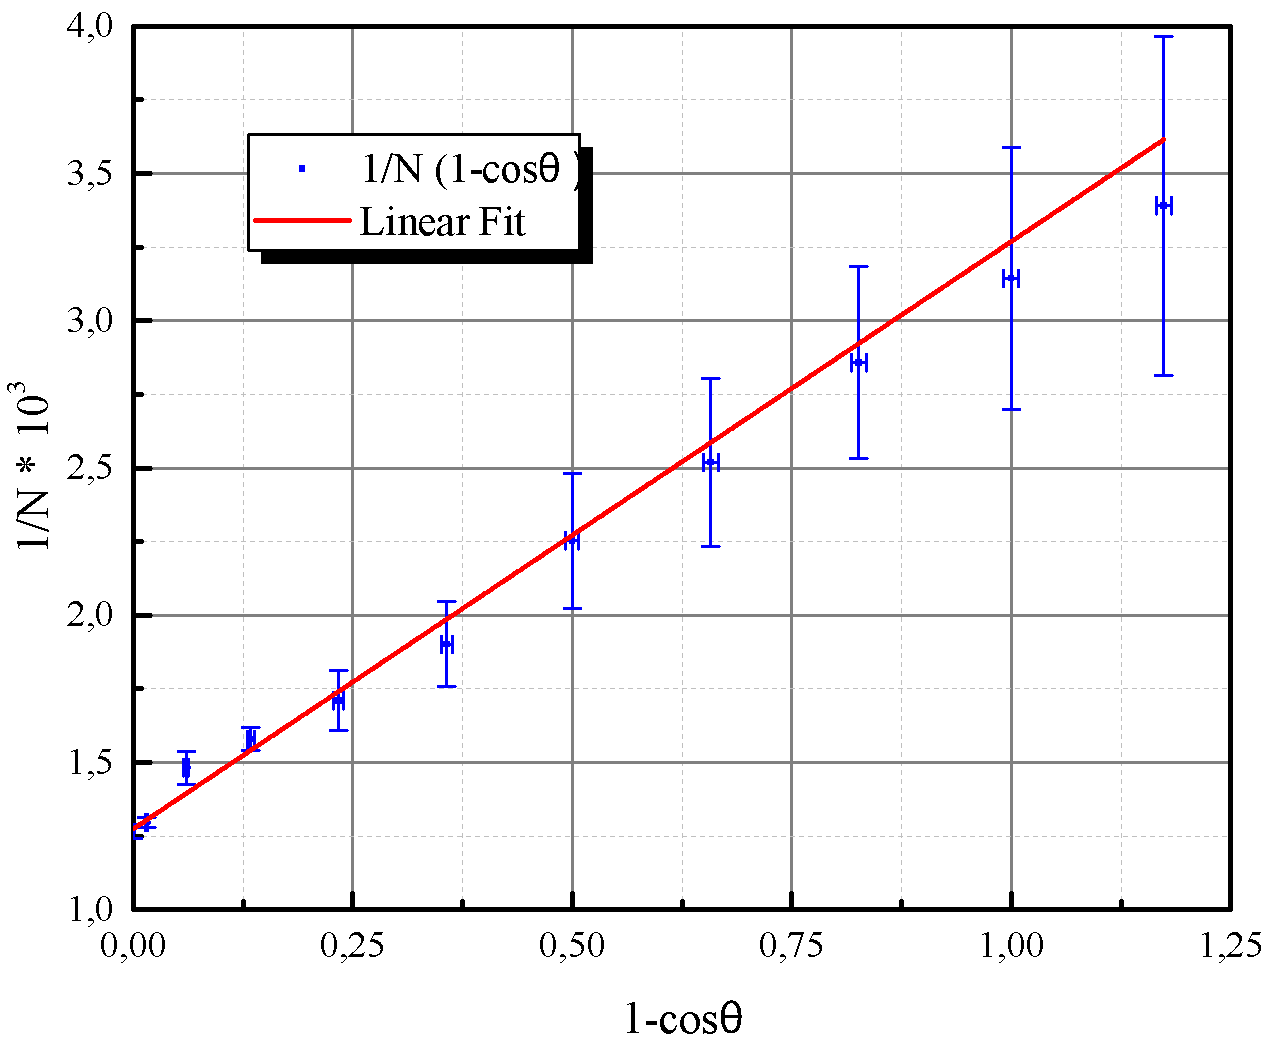
\includegraphics[width=.9\textwidth]{graph1.jpg}
	\end{center}
\end{figure}

Теперь построим графики зависимости ЭДС Холла $\mathcal{E}_X$ от $B$ при различных токах $I$, текущих через образец.

\begin{figure}[H]
	\begin{center}	\includegraphics[width=1\textwidth]{tabliza2.jpg}
	\end{center}
\end{figure}

\begin{figure}[H]
	\begin{center}	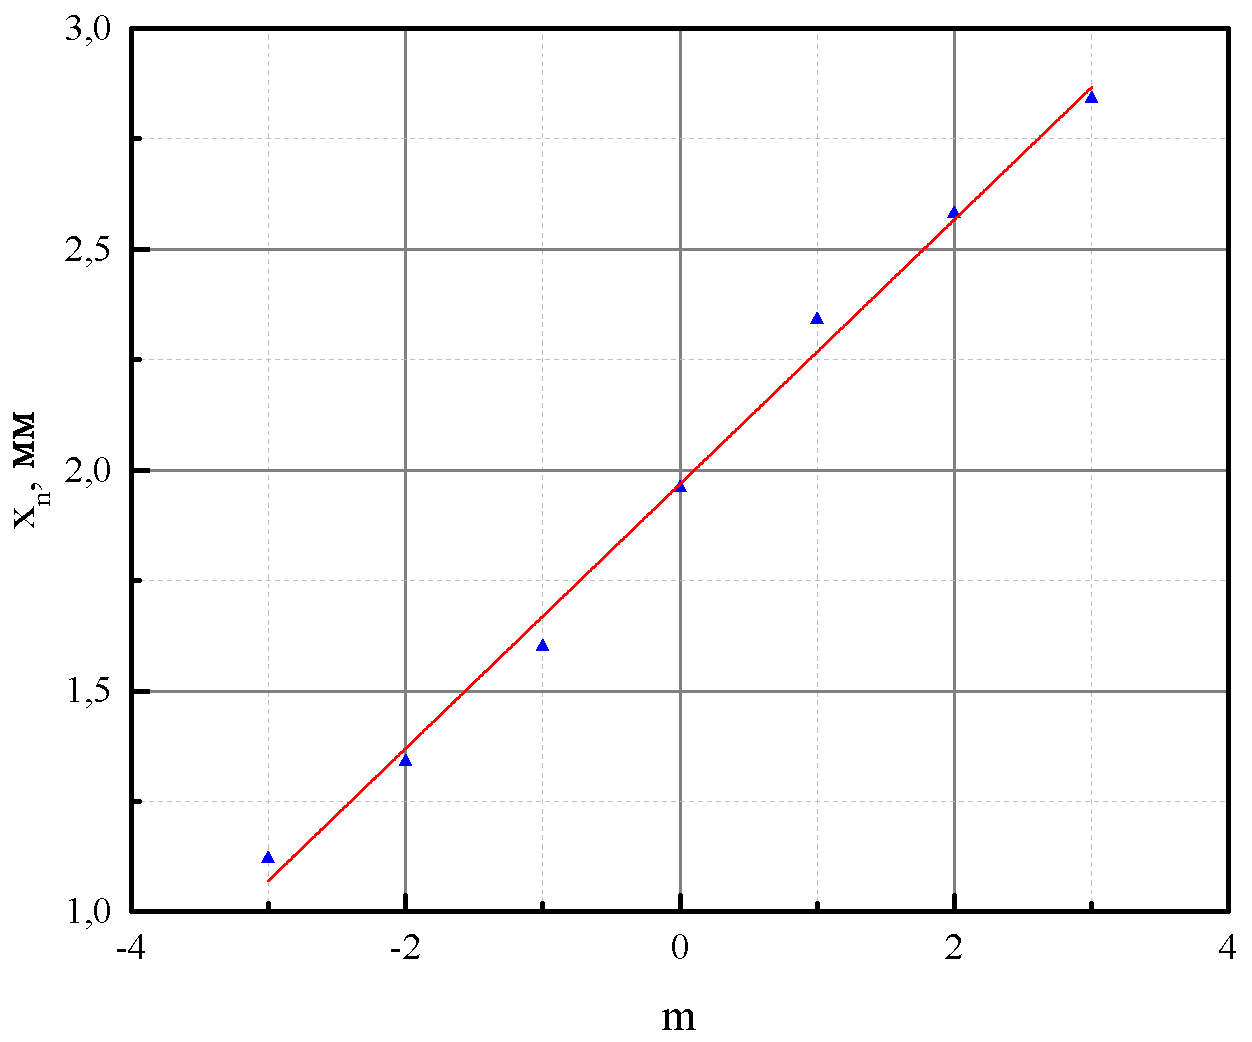
\includegraphics[width=1\textwidth]{graph2.jpg}
	\end{center}
\end{figure}
Теперь рассмотрим формулу $(1)$:
\[\mathcal{E}_X = R_x \cdot \frac{I \cdot B}{a} \Rightarrow \frac{\mathcal{E}_X}{B} = \frac{R_X}{a} \cdot I\]
Построим график зависимости $K = \frac{\mathcal{E}_X}{B}$ от $I$, при помощи коэффициента пропорциональности этой линейной зависимости найдем значение постоянной Холла.
\begin{figure}[H]
	\begin{center}	\includegraphics[width=.4\textwidth]{tabliza3.jpg}
	\end{center}
\end{figure}

\begin{figure}[H]
	\begin{center}	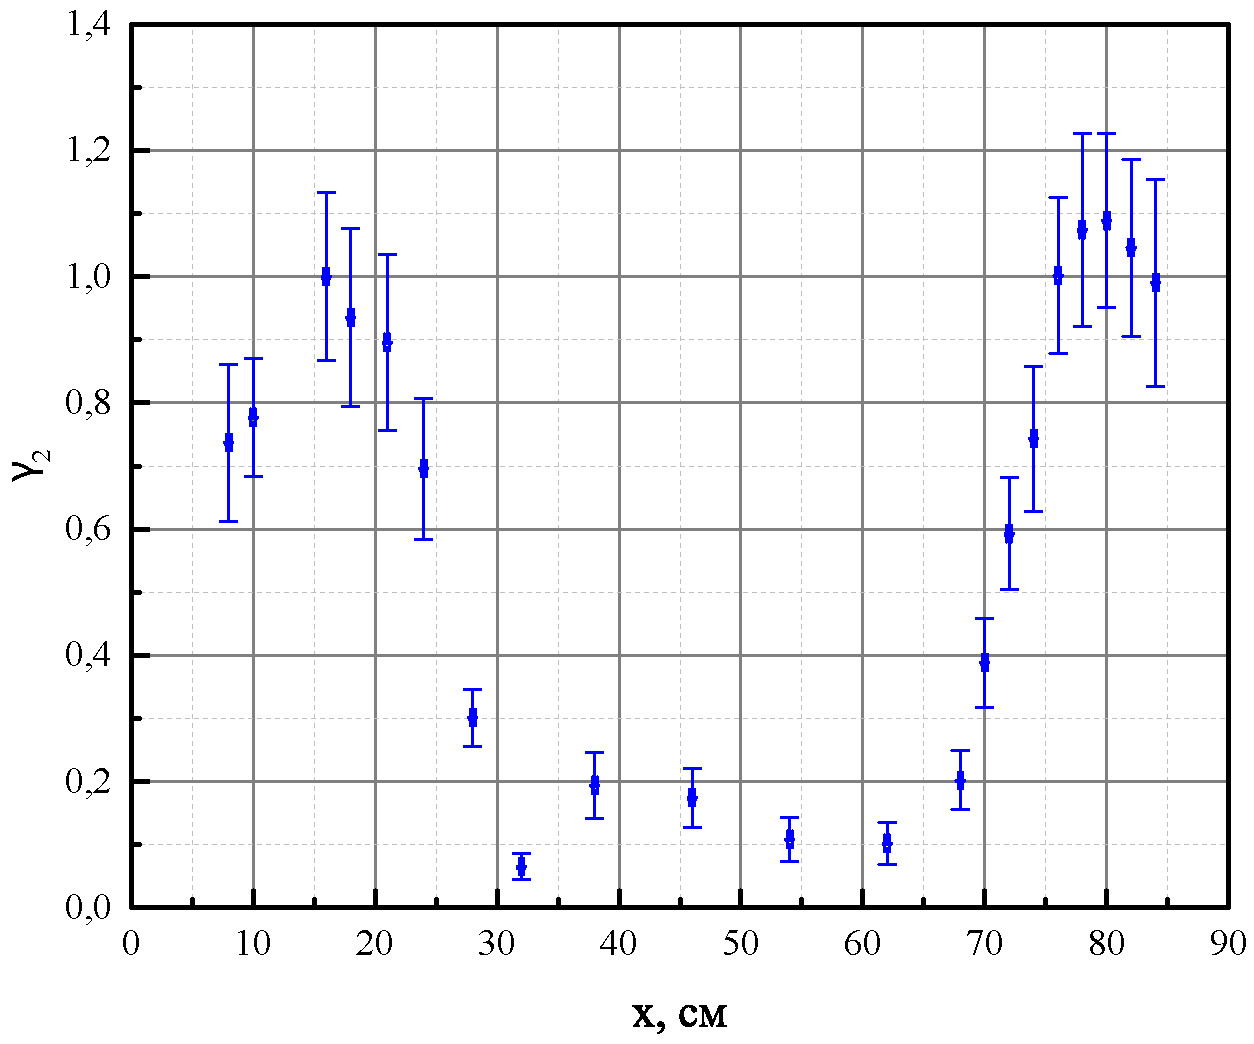
\includegraphics[width=1\textwidth]{graph3.jpg}
	\end{center}
\end{figure}

Получается коэффициент пропорциональности равен $k = 198,86 \frac{\text{мкВ}}{\text{мА} \cdot \text{Тл}}$.

Значит, $R_X = a \cdot k = 437,49 \cdot 10^{-6} \frac{B \cdot \text{м}}{A \cdot \text{Тл}}$.

Теперь разберёмся с характером проводимости

\begin{figure}[H]
	\begin{center}	\includegraphics[width=1\textwidth]{last.jpg}
	\end{center}
\end{figure}

Из вышеприведённого рисунка видно, что Холловские частицы двигаются к клемме $4$. Теперь посмотрим показания вольтметра без магнитного поля и с магнитным полем. $U_{\text{без}} = 20$ мкВ $ U_{\text{с}} = 125$ мкВ. Знак у напряжения положительны, а это значит, что разность потенциалов $\varphi_3 - \varphi_4 > 0$, из чего следует, что Холловское поле направлено от клеммы 3 к клемме 4. Такое возможно только если Холловскими частицами являются электроны.

Найдем теперь концентрацию электронов в образце $n = \frac{1}{R_x \cdot e} = 1428,6 \cdot 10^{19} \text{м}^{-3}$.

Теперь, подключив потенциальные концы $3$ и $5$ к вольтметру, измерим падение напряжения $U_{3,5}$ при токе через образец равном $I_0 = 1$ мА. Получилось $U_{3,5} = 1,74$ мВ. Тогда по формуле $(2)$ найдем значение проводимости материала образца. $\sigma = 313,5 \frac{1}{\text{Ом} \cdot \text{м}}$.

И наконец, зная значения проводимости и концентрации, найдем подвижность электронов в образце по формуле
\[b = \frac{\sigma}{e \cdot n} = 1372 \frac{\text{см}^2}{B \cdot \text{с}} \]

Итоговая таблица

\begin{figure}[H]
	\begin{center}	\includegraphics[width=1\textwidth]{tabliza4.jpg}
	\end{center}
\end{figure}
\section{Вывод}
В ходе работы был исследован эффект Холла в полупроводнике, сделанном из Германия, измерены его основные параметры, такие как: постоянная Холла, подвижность, концентрация носителей тока, а также проводимость, также был исследован характер проводимости, выяснено какие частицы в нашем случае являются Холловскими. Значения по порядку совпадают со справочными, однако некоторые из них достаточно сильно отличаются от табличных. Это различие вызвано тем, что данный полупроводник имеет в себе примеси, которые, как и было получено, могут сильно изменить характеристики материала.
\end{document}